\documentclass[xcolor=dvipsnames,t,aspectratio=169]{beamer}

\usecolortheme{rose}
\usecolortheme{dolphin}
\usetheme{Boadilla}

\input{../../templates/slides/imports}
\input{../../templates/slides/settings}
\input{../../templates/slides/commands}

\titlegraphic{
    \includegraphics[scale = 0.5]{../../templates/slides/logo}
}

\logo{
\begin{tikzpicture}[overlay,remember picture]
\node[xshift=-.75cm, yshift=-1cm] at (current page.30){
    \includegraphics[width=0.1\textwidth]{../../templates/slides/logo}};
\end{tikzpicture}
}
\usetikzlibrary{positioning}

\newcommand{\highlight}[1]{{\color{nes_dark_orange} #1}}

\title{Visualização de dados e EDA}

\author{Eduardo Adame}

\date{{\color{nes_dark_purple}\textbf{Ciência de Dados}\\[0.5em] 10 de abril de 2026 }}

\begin{document}

\frame[plain]{\titlepage}
\setcounter{framenumber}{0}


% ============================================================
\section{Motivação}
% ============================================================

\begin{frame}[c]{Por que visualizar?}

Antes de modelar, precisamos \highlight{entender} os dados — e o olho humano é extraordinariamente bom em detectar padrões, outliers e estruturas que estatísticas resumidas escondem.

\begin{columns}
\column{0.48\textwidth}
\textbf{\color{nes_dark_purple}Quarteto de Anscombe (1973)}
\begin{itemize}
    \item Quatro datasets com \highlight{mesma média, variância e correlação}
    \item Estruturas completamente diferentes
    \item Invisíveis sem visualização
\end{itemize}

\column{0.48\textwidth}
\textbf{\color{nes_dark_purple}Datasaurus Dozen (2017)}
\begin{itemize}
    \item 13 datasets com \highlight{estatísticas idênticas}
    \item Formas radicalmente distintas
    \item Moral: \texttt{df.describe()} não é suficiente
\end{itemize}
\end{columns}

\vspace{0.8em}

\begin{display}[Regra de ouro da EDA]
Nunca ajuste um modelo antes de plotar os dados.
\end{display}

\end{frame}

\begin{frame}[c]{Por que visualizar? Quarteto de Anscombe (1973)}
\begin{figure}
    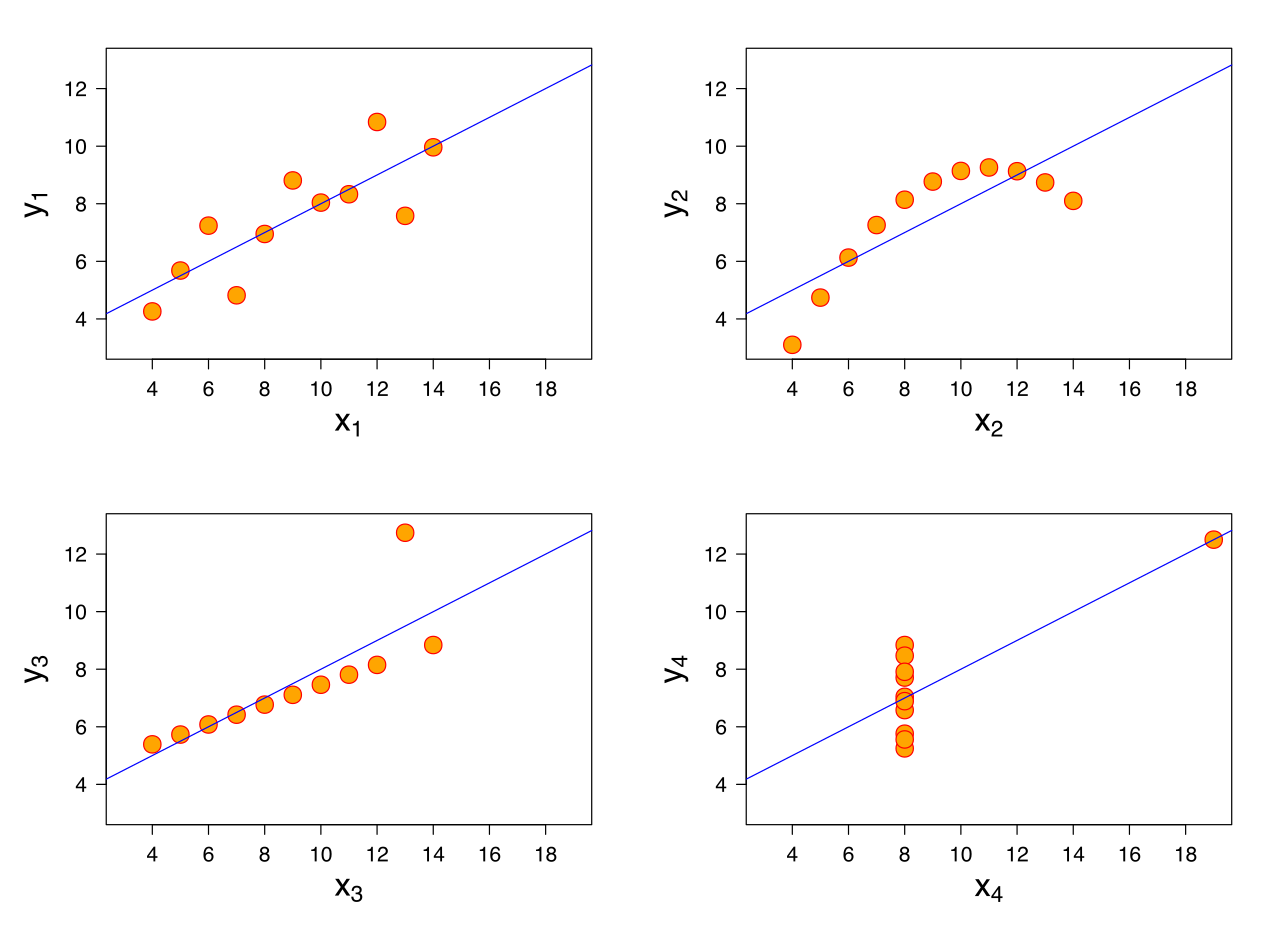
\includegraphics[height=.9\textheight]{anscombe.png}
\end{figure}
\end{frame}

\begin{frame}[c]{Por que visualizar? Datasaurus Dozen (2017)}
\begin{figure}
    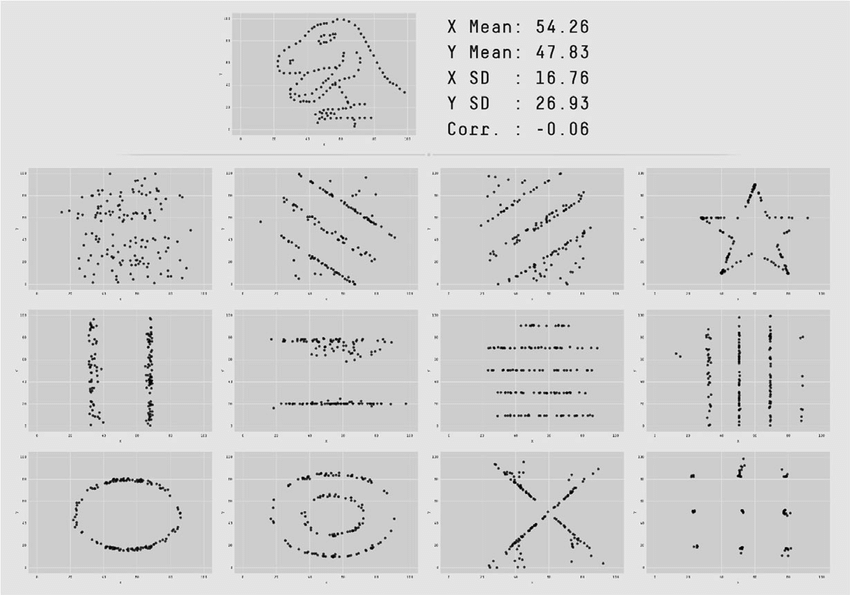
\includegraphics[height=.9\textheight]{datasaurus.png}
\end{figure}
\end{frame}

\begin{frame}[c]{O ecossistema de visualização em Python}

% Sugestão de imagem: diagrama de camadas mostrando Matplotlib na base, Seaborn e Pandas.plot sobre ele, e Plotly/Altair como alternativas independentes

\begin{columns}
\column{0.48\textwidth}
\textbf{\color{nes_dark_purple}Baseadas em Matplotlib}
\begin{itemize}
    \item \texttt{matplotlib} — controle total, verboso
    \item \texttt{pandas .plot} — atalho rápido para DataFrames
    \item \texttt{seaborn} — estatística + estética
\end{itemize}

\column{0.48\textwidth}
\textbf{\color{nes_dark_purple}Independentes}
\begin{itemize}
    \item \texttt{plotly} — interativo, web-ready
    \item \texttt{altair} — gramática declarativa (Vega-Lite)
\end{itemize}
\end{columns}

\vspace{0.8em}

\begin{display}[Qual usar?]
Exploração rápida: \texttt{pandas} ou \texttt{seaborn}. Publicação: \texttt{matplotlib}. Dashboards: \texttt{plotly}. Artigos e gramática limpa: \texttt{altair}.
\end{display}

\end{frame}


% ============================================================
\section{Pandas .plot}
% ============================================================

\begin{frame}[c, fragile]{Visualização direto do DataFrame}

\begin{code}[Tipos básicos com .plot]{python}
import pandas as pd
df["nota"].plot(kind="hist", bins=20, title="Distribuição de notas")
df["nota"].plot(kind="box")
df.plot(kind="scatter", x="idade", y="nota")
df["turma"].value_counts().plot(kind="bar")
\end{code}

\begin{code}[Atalhos convenientes]{python}
df["nota"].plot.hist(bins=20)
df["nota"].plot.kde()          # densidade estimada
df.plot.scatter(x="x", y="y")
\end{code}

\begin{itemize}
    \item Retorna um objeto \texttt{matplotlib Axes} — customizável depois
    \item \texttt{kind}: \texttt{"line"}, \texttt{"bar"}, \texttt{"barh"}, \texttt{"hist"}, \texttt{"box"}, \texttt{"kde"}, \texttt{"scatter"}, \texttt{"pie"}
\end{itemize}

\end{frame}


\begin{frame}[c, fragile]{Agrupando e plotando}

\begin{code}[Comparar distribuições por grupo]{python}
df.groupby("turma")["nota"].plot(kind="kde", legend=True)
# Múltiplas colunas lado a lado
df[["nota_p1", "nota_p2", "nota_p3"]].plot(kind="box")
# Série temporal
df.set_index("data")["vendas"].plot(kind="line")
\end{code}

\begin{itemize}
    \item \texttt{subplots=True} cria um painel por coluna
    \item \texttt{figsize=(largura, altura)} controla o tamanho
    \item Passe \texttt{ax=ax} para compor com Matplotlib
\end{itemize}

\begin{display}[Quando usar .plot]
Ideal para exploração rápida e prototipagem. Para publicação, migre para Matplotlib ou Seaborn.
\end{display}

\end{frame}


% ============================================================
\section{Matplotlib}
% ============================================================

\begin{frame}[c, fragile]{Anatomia de uma figura Matplotlib}

% Sugestão de imagem: diagrama rotulado com Figure, Axes, Axis, Title, xlabel, ylabel, legend — estilo "anatomia oficial"

\begin{code}[Interface orientada a objetos (recomendada)]{python}
import matplotlib.pyplot as plt
fig, ax = plt.subplots(figsize=(8, 4))
ax.scatter(df["idade"], df["nota"], alpha=0.5, color="#5B2D8E")
ax.set_xlabel("Idade")
ax.set_ylabel("Nota final")
ax.set_title("Nota vs. Idade")
ax.axhline(6.0, color="red", linestyle="--", label="Aprovação")
ax.legend()
fig.tight_layout()
\end{code}

\begin{itemize}
    \item \texttt{fig} controla tamanho, resolução e exportação
    \item \texttt{ax} controla o conteúdo do gráfico
    \item Prefira a interface OO à interface \texttt{plt.xxx()} em scripts
\end{itemize}

\end{frame}


\begin{frame}[c, fragile]{Grids e painéis}

\begin{code}[Subplots com layout automático]{python}
fig, axes = plt.subplots(nrows=2, ncols=2, figsize=(10, 7))
axes[0, 0].hist(df["nota_p1"].dropna(), bins=20, color="#5B2D8E")
axes[0, 1].hist(df["nota_p2"].dropna(), bins=20, color="#E8650A")
axes[1, 0].hist(df["nota_p3"].dropna(), bins=20, color="#2D8E5B")
axes[1, 1].boxplot([df["nota_p1"].dropna(),
                    df["nota_p2"].dropna(),
                    df["nota_p3"].dropna()])
fig.suptitle("Distribuição por prova", fontsize=14)
fig.tight_layout()
\end{code}

\begin{code}[Layout com proporções customizadas]{python}
fig, (ax1, ax2) = plt.subplots(1, 2, figsize=(12, 4),
                                gridspec_kw={"width_ratios": [2, 1]})
\end{code}

\end{frame}


\begin{frame}[c, fragile]{Exportando figuras}

\begin{code}[Salvando em diferentes formatos]{python}
fig.savefig("figura.png", dpi=150, bbox_inches="tight")
fig.savefig("figura.pdf", bbox_inches="tight")   # vetorial
fig.savefig("figura.svg", bbox_inches="tight")   # web
\end{code}

\begin{itemize}
    \item \texttt{dpi=150} ou \texttt{dpi=300} para qualidade de publicação
    \item \texttt{bbox\_inches="tight"} evita cortes nas bordas
    \item \texttt{transparent=True} para fundo transparente
    \item PDF e SVG são \highlight{vetoriais} — preferíveis para artigos
\end{itemize}

\begin{display}[Dica de reprodutibilidade]
Salve as figuras programaticamente no pipeline — nunca use "Print Screen".
\end{display}

\end{frame}


% ============================================================
\section{Seaborn}
% ============================================================

\begin{frame}[c, fragile]{Seaborn — estatística com estética}

Seaborn é construído sobre Matplotlib e oferece \highlight{tipos de gráfico estatísticos} com uma API de alto nível.

\begin{code}[Importando e configurando tema]{python}
import seaborn as sns
sns.set_theme(style="whitegrid", palette="muted")
\end{code}

\begin{columns}
\column{0.48\textwidth}
\textbf{\color{nes_dark_purple}Distribuições}
\begin{itemize}
    \item \texttt{histplot} — histograma + KDE
    \item \texttt{kdeplot} — densidade
    \item \texttt{boxplot} / \texttt{violinplot}
    \item \texttt{ecdfplot} — função acumulada
\end{itemize}

\column{0.48\textwidth}
\textbf{\color{nes_dark_purple}Relações e categorias}
\begin{itemize}
    \item \texttt{scatterplot} / \texttt{lineplot}
    \item \texttt{barplot} — média + IC
    \item \texttt{heatmap} — correlação
    \item \texttt{pairplot} — matriz de dispersão
\end{itemize}
\end{columns}

\end{frame}


\begin{frame}[c, fragile]{Gráficos distribucionais}

\begin{code}[Histograma com KDE e separação por grupo]{python}
import seaborn as sns
sns.histplot(data=df, x="nota", hue="turma",
             kde=True, bins=20, alpha=0.5)
sns.boxplot(data=df, x="turma", y="nota",
            order=["A", "B", "C"])
sns.violinplot(data=df, x="turma", y="nota",
               inner="quartile", palette="muted")
\end{code}

\begin{itemize}
    \item \texttt{hue} separa grupos por cor automaticamente
    \item \texttt{violinplot} mostra distribuição \highlight{e} quartis simultaneamente
    \item Todos retornam \texttt{Axes} — customizáveis com Matplotlib
\end{itemize}

\end{frame}


\begin{frame}[c, fragile]{Relações e matriz de correlação}

\begin{code}[Scatter com regressão e correlação]{python}
sns.regplot(data=df, x="idade", y="nota", scatter_kws={"alpha": 0.4})
# Mapa de calor da correlação
corr = df[["nota_p1", "nota_p2", "nota_p3", "idade"]].corr()
sns.heatmap(corr, annot=True, fmt=".2f",
            cmap="coolwarm", vmin=-1, vmax=1)
# Matriz de dispersão completa
sns.pairplot(df[["nota_p1", "nota_p2", "nota_p3"]], diag_kind="kde")
\end{code}

\begin{display}[Interpretando o heatmap]
Valores próximos de $+1$: correlação positiva forte.
Próximos de $0$: sem relação linear.
Próximos de $-1$: correlação negativa forte.
\end{display}

\end{frame}


\begin{frame}[c, fragile]{\texttt{FacetGrid} — facetamento por variável}

\begin{code}[Replicar gráfico por subgrupo]{python}
g = sns.FacetGrid(df, col="turma", height=3, aspect=1.2)
g.map(sns.histplot, "nota", bins=15, kde=True)
g.set_axis_labels("Nota", "Frequência")
g.set_titles("Turma {col_name}")
\end{code}

\begin{code}[catplot — interface de alto nível]{python}
sns.catplot(data=df, x="turma", y="nota",
            hue="aprovado", kind="box",
            height=4, aspect=1.5)
\end{code}

\begin{itemize}
    \item \texttt{FacetGrid} é a base de \texttt{catplot}, \texttt{relplot}, \texttt{displot}
    \item Permite criar \highlight{painéis condicionais} com uma linha
\end{itemize}

\end{frame}


% ============================================================
\section{Plotly}
% ============================================================

\begin{frame}[c, fragile]{Plotly — visualizações interativas}

Plotly gera gráficos \highlight{interativos} baseados em HTML/JavaScript — ideais para dashboards e relatórios web.

\begin{code}[Plotly Express — API rápida]{python}
import plotly.express as px
fig = px.histogram(df, x="nota", color="turma",
                   nbins=20, barmode="overlay",
                   title="Distribuição de notas por turma")
fig.show()
fig = px.scatter(df, x="idade", y="nota",
                 color="turma", hover_data=["nome"],
                 trendline="ols")
fig.show()
\end{code}

\begin{itemize}
    \item \texttt{hover\_data} — dados exibidos ao passar o mouse
    \item \texttt{color}, \texttt{facet\_col}, \texttt{animation\_frame} — encoding declarativo
\end{itemize}

\end{frame}


\begin{frame}[c, fragile]{Plotly — exportação e personalização}

\begin{code}[Exportar para HTML e imagem]{python}
fig.write_html("grafico.html")           # interativo
fig.write_image("grafico.png", scale=2)  # requer kaleido

# Customização com update_layout
fig.update_layout(
    template="plotly_white",
    font=dict(family="Arial", size=13),
    legend=dict(orientation="h", y=-0.2),
)
fig.update_traces(marker_opacity=0.6)
\end{code}

\begin{display}[Quando usar Plotly]
Relatórios interativos, dashboards (Dash/Streamlit) e quando o leitor precisará explorar os dados. Para publicação estática, prefira Matplotlib ou Seaborn.
\end{display}

\end{frame}


% ============================================================
\section{Altair}
% ============================================================

\begin{frame}[c, fragile]{Altair — gramática de visualização}

Altair implementa a \highlight{gramática Vega-Lite}: você declara o \emph{mapeamento} entre dados e elementos visuais, e a biblioteca cuida do resto.

\begin{code}[Conceito: encoding de canais]{python}
import altair as alt
alt.Chart(df).mark_point().encode(
    x="idade:Q",      # Q = quantitativo
    y="nota:Q",
    color="turma:N",  # N = nominal
    tooltip=["nome", "nota", "turma"]
)
\end{code}
\end{frame}

\begin{frame}[c, fragile]{Altair — gramática de visualização}
\begin{columns}
\column{0.48\textwidth}
\textbf{\color{nes_dark_purple}Tipos de dados}
\begin{itemize}
    \item \texttt{Q} — quantitativo
    \item \texttt{N} — nominal (categórico)
    \item \texttt{O} — ordinal
    \item \texttt{T} — temporal
\end{itemize}

\column{0.48\textwidth}
\textbf{\color{nes_dark_purple}Marcas (\texttt{mark\_*})}
\begin{itemize}
    \item \texttt{point}, \texttt{line}, \texttt{bar}
    \item \texttt{area}, \texttt{rect}, \texttt{rule}
    \item \texttt{boxplot}, \texttt{errorband}
\end{itemize}
\end{columns}

\end{frame}


\begin{frame}[c, fragile]{Altair — composição e interatividade}

\begin{code}[Camadas e painéis]{python}
base = alt.Chart(df)
pontos = base.mark_point(opacity=0.5).encode(
    x="idade:Q", y="nota:Q", color="turma:N"
)
linha = base.mark_rule(color="red").encode(
    y=alt.datum(6.0)          # linha de aprovação
)
grafico = (pontos + linha).properties(width=400, height=300)
# Facetamento
grafico.facet(column="turma:N")
\end{code}
\end{frame}

\begin{frame}[c, fragile]{Altair — composição e interatividade}
\begin{code}[Interatividade com uma linha]{python}
selecao = alt.selection_point(fields=["turma"])
pontos.add_params(selecao).encode(
    opacity=alt.condition(selecao, alt.value(1), alt.value(0.1))
)
\end{code}

\end{frame}


% ============================================================
\section{Colormaps e tipos de dados}
% ============================================================

\begin{frame}[c]{Colormaps — escolha certa para cada dado}

% Sugestão de imagem: barra de cores mostrando exemplos de cada categoria (sequencial, divergente, qualitativo) lado a lado

\begin{columns}
\column{0.33\textwidth}
\textbf{\color{nes_dark_purple}Sequencial}\\
Dados ordenados com zero natural
\begin{itemize}
    \item \texttt{viridis}, \texttt{plasma}
    \item \texttt{Blues}, \texttt{YlOrRd}
    \item Claro $\to$ escuro
\end{itemize}

\column{0.33\textwidth}
\textbf{\color{nes_dark_purple}Divergente}\\
Dados com ponto médio significativo
\begin{itemize}
    \item \texttt{RdBu}, \texttt{coolwarm}
    \item \texttt{PuOr}, \texttt{BrBG}
    \item Ex: correlações, desvios
\end{itemize}

\column{0.33\textwidth}
\textbf{\color{nes_dark_purple}Qualitativo}\\
Categorias sem ordem
\begin{itemize}
    \item \texttt{tab10}, \texttt{Set2}
    \item Seaborn \texttt{"muted"}
    \item Ex: turmas, classes
\end{itemize}
\end{columns}

\vspace{0.8em}

\begin{display}[Acessibilidade]
Evite \texttt{jet} e \texttt{rainbow} — enganam o olho e são inacessíveis para daltônicos. \texttt{viridis} é perceptualmente uniforme e seguro.
\end{display}

\end{frame}


\begin{frame}[c]{Qual gráfico para qual tipo de dado?}

% Sugestão de imagem: tabela visual "cheat sheet" com ícones de cada tipo de gráfico

\begin{columns}
\column{0.5\textwidth}
\textbf{\color{nes_dark_purple}Uma variável}
\begin{itemize}
    \item Contínua: \texttt{histplot}, \texttt{kdeplot}, \texttt{boxplot}
    \item Discreta / categórica: \texttt{countplot}, \texttt{barplot}
\end{itemize}

\vspace{0.5em}
\textbf{\color{nes_dark_purple}Duas variáveis}
\begin{itemize}
    \item Contínua $\times$ contínua: \texttt{scatter}, \texttt{hexbin}, \texttt{kde2d}
    \item Categórica $\times$ contínua: \texttt{box}, \texttt{violin}, \texttt{strip}
    \item Categórica $\times$ categórica: \texttt{heatmap}, mosaico
\end{itemize}

\column{0.5\textwidth}
\textbf{\color{nes_dark_purple}Muitas variáveis}
\begin{itemize}
    \item Matriz: \texttt{pairplot}, \texttt{heatmap} de correlação
    \item Terceira variável: cor, tamanho, forma, faceta
\end{itemize}

\vspace{0.5em}
\textbf{\color{nes_dark_purple}Temporal}
\begin{itemize}
    \item \texttt{lineplot}, área empilhada
    \item Sazonalidade: \texttt{heatmap} mês $\times$ ano
\end{itemize}
\end{columns}

\end{frame}


\begin{frame}[c]{EDA — checklist prático}

\begin{columns}
\column{0.5\textwidth}
\textbf{\color{nes_dark_purple}1. Inspecionar}
\begin{itemize}
    \item \texttt{df.info()}, \texttt{df.describe()}
    \item Tipos corretos? NaN onde?
\end{itemize}

\textbf{\color{nes_dark_purple}2. Univariada}
\begin{itemize}
    \item Distribuição de cada variável
    \item Outliers visíveis?
    \item Simetria, caudas, modas
\end{itemize}


\textbf{\color{nes_dark_purple}3. Bivariada}
\begin{itemize}
    \item Correlações entre numéricas
    \item Variáveis numéricas por categoria
\end{itemize}

\column{0.5\textwidth}
\textbf{\color{nes_dark_purple}4. Multivariada}
\begin{itemize}
    \item \texttt{pairplot} ou \texttt{heatmap}
    \item Adicionar cor/faceta por grupo
\end{itemize}


\textbf{\color{nes_dark_purple}5. Temporal (se houver)}
\begin{itemize}
    \item Tendência, sazonalidade
    \item Quebras estruturais
\end{itemize}


\textbf{\color{nes_dark_purple}6. Comunicar}
\begin{itemize}
    \item Título informativo
    \item Eixos rotulados com unidades
    \item Colormap adequado
\end{itemize}
\end{columns}

\begin{display}[Objetivo da EDA]
Gerar hipóteses. A confirmação vem depois, com modelos.
\end{display}

\end{frame}


\begin{frame}[c, noframenumbering, plain]
    \frametitle{~}
        \vfill
        \begin{center}
            {\Huge Obrigado!}\vspace{1.5em}\\
            {\Large \highlight{Alguma dúvida?}}\\
        \end{center}
        \vfill
        \begin{center}
            {\small Agora vamos para os exercícios!}
        \end{center}
\end{frame}

\end{document}